\documentclass[12pt,a4paper]{article}
% 如果需要中文支持，推荐使用xeCJK + 字体设置
% \usepackage{xeCJK}
% \setCJKmainfont{SimSun}  % 示例：宋体，可根据系统字体情况更换
\usepackage{ctex}
\setlength{\parindent}{2em}
\setlength{\parskip}{0pt} % 确保段落之间没有额外的空行间距


\usepackage{amsmath}      % 数学公式（如有需要）
\usepackage{graphicx}     % 插图
\usepackage{geometry}     % 调整页边距
\usepackage{fancyhdr}     % 自定义页眉页脚
\usepackage{indentfirst}  % 中文首行缩进
\usepackage{calc}         % 允许做长度运算(测量文字宽度等)
\usepackage{titlesec}
\usepackage{booktabs} % 解决 \midrule 和 \bottomrule 报错
\usepackage{enumitem} % 支持自定义列表格式
\usepackage{float}    % 支持强制浮动位置
\usepackage{siunitx}
\usepackage{wrapfig}

% 设置 \section 级标题为：加粗、大字号（如 \Large）
\titleformat{\section}
	{\bfseries\large}    % 标题自身的格式
	{\thesection}        % 标题编号的显示方式
	{1em}                % 编号与标题文字之间的间距
	{}                   % 在标题文字前后可插入额外代码，此处为空
	
% 设置 \subsection 级标题为：加粗、中等字号（如 \normalsize）
\titleformat{\subsection}
	{\bfseries\normalsize}
	{\thesubsection}
	{1em}
{}

% 页面设置（可根据需要微调）
\geometry{
	left=2cm,
	right=2cm,
	top=1cm,
	bottom=1.5cm
}

% 不需要过大的行距，使用较接近单倍行距的设置
\renewcommand{\baselinestretch}{1.2}

% 仅在页脚居中显示页码，页眉保持为空
\pagestyle{fancy}
\fancyhf{}  % 清空默认的页眉页脚
\fancyfoot[C]{\thepage}
\renewcommand{\headrulewidth}{0pt}
\renewcommand{\footrulewidth}{0pt}

% 首行缩进2字符(中文习惯)
% \setlength{\parindent}{0pt}
\setlength{\leftskip}{2em}
\setlength{\parindent}{2em}

\begin{document}
	%-------------------------------------------------------
	% 1 并排两个minipage：左标题、右校徽
	%   - 0.65\textwidth + 0.35\textwidth = \textwidth
	%   - 如果校徽过大或过小，可改宽度，如 0.25\textwidth、0.3\textwidth 等
	%   - 如果想让标题更大，可将 \Huge 改成 \huge 或 \LARGE
	%-------------------------------------------------------
	\noindent
	\hspace{-2em}
	\begin{minipage}[c]{0.65\textwidth}
		\raggedright
		{\fontsize{35pt}{55pt}\selectfont 物理实验报告}
	\end{minipage}
	\begin{minipage}[c]{0.35\textwidth}
		\raggedleft
		% 强制把校徽拉大到 0.35\textwidth 宽度 (高度自动匹配)
		% 若想指定高度,可用 "height=3cm" 等. 二选一即可.
		
\includegraphics[width=\linewidth, trim={20cm 20cm 20cm 20cm}, clip]{university_logo.png}
	\end{minipage}

	\vspace{-1em}
	

	%下方画两条分割线，并在两线之间写学号、姓名、日期、时间
	
	\hrule
	\vspace{0.6em}
	\noindent
	\begin{tabular}{l l l l}
    学号：12411434 & 姓名：{郑宇轩} &
    日期：2025.11.28 & 时间：周五下午
	\end{tabular}
	\vspace{0.4em}
	\par
	\hrule

	
	\section*{\textbf{一. 实验名称：测量螺线管的磁场}}
	
	\section*{\textbf{二. 实验目的}}
	\begin{enumerate}
		\item 学习测量交变磁场的一种方法，加深理解磁场的一些特性及电磁感应定律。
	\end{enumerate}

	\section*{\textbf{{三. 实验原理}}}

	\begin{enumerate}

	\item \textbf{有限长载流直螺线管的磁场}
	
	图1左是一个长为2l，匝数为N的单层密绕的直螺线管产生的磁场。当导线中流过电流I时，由毕奥-萨伐尔定律可以计算出在轴线上某一点P的磁感应强度为
		\begin{equation}
		B = \frac{\mu_0 n I}{2} \left\{ \frac{x+l}{\sqrt{R^2+(x+l)^2}} - \frac{x-l}{\sqrt{R^2+(x-l)^2}} \right\}
		\end{equation}
		其中 $\mu_0 = 4\pi\times10^{-7}\mathrm{N/A^2}$，$n = \dfrac{N}{2l}$ 为单位长度上的线圈数，$R$ 为线圈管半径，$x$ 为 P 点到线圈管中心处的距离。
		\begin{figure}[htbp]
			\centering
			
\includegraphics[width=0.40\textwidth]{1.jpg}
			
\includegraphics[width=0.40\textwidth]{2.jpg}
			\caption{实验原理图}
			\label{fig:chart1}
			\end{figure}
		图1左同时给出 $B$ 随 $x$ 的分布曲线。由曲线显示，在线圈管内部磁场近于均匀，只在端点附近磁感应强度才显著下降。当 $l \gg R$ 时，$B = \mu_0 n I$ 即场点的坐标 $x$ 对内部磁场无影响，而在线圈管两端，$B = \frac{1}{2}\mu_0 n I$为内部 $B$ 值的一半。无限长、密绕的直线线圈是实验室中常用的产生均匀磁场的理想装置。
	
	\item \textbf{探测线圈法测量磁场}
	
	本实验采用电磁感应原理测量直螺线管中产生的交变磁场。图1右是实验装置的示意图。当低频交流电流通过螺线管产生磁场时，检测线圈中感应出的电压 \(V\) 与磁感应强度 \(B\) 的关系可写为
	\begin{equation}\label{eq:B}
	B = \frac{V}{2\pi^2N_1r_1^2f} \tag{2}
	\end{equation}
	其中，\(N_1\) 为螺线管的匝数，\(r_1\) 为检测线圈半径，\(f\) 为交流电频率。在测量过程中如始终保持 A 和 $A_1$ 在同一轴线上。

	
	\end{enumerate}
	
	\section*{\textbf{{四. 实验仪器}}}
	螺线管套件，示波器，信号发生器，电阻，导线

	\section*{\textbf{{五. 实验内容}}}


	\begin{enumerate}
	\item 研究螺线管中磁感应强度 $B$与电流$I$和感生电动势$V$之间的关系，测量螺线管中的磁感应强度
	
	\begin{enumerate}
	
	\item 记录参数：螺线管A的半径$R$、长度$2L$、总匝数$N$，探测线圈A1 的半径$r_1$和总匝数$N_1$（参数由实验仪器面板给出）。\\
	\item  按图1右接好线路。需要注意的是，本实验螺线管串联 $1\Omega$的电阻，通过探测电阻两端电压，可以得到输出电流。 \\
	\item A和A1两个中心点的距离代表磁场场点坐标$x$，其值由装置中的直尺读出。取$x=0$（中心位置），低频信号发生器频率分别选取为$f=4000\mathrm{Hz},2000\mathrm{Hz},1000\mathrm{Hz}$，调节信号输出使输出电流从$10.0$mA至$40.0$mA，每隔$5.0$mA记录相应的感生电动势V。 \\
	\item 取$x=l$（管口位置），频率和电流分别取三组数值：$f=4000\mathrm{Hz},I=10.0\mathrm{mA};f=2000\mathrm{Hz},I=20.0\mathrm{mA};f=1000\mathrm{Hz},I=40.0\mathrm{mA}$，测出对应的 V值。从测量结果中可以得出什么结论？\\
	\item 从以上测量数据中取出$x=0$，$f=1000\mathrm{Hz}$，$I=40.0\mathrm{mA}$和对应的$V$值，再取$x=l$，$f=1000\mathrm{Hz}$，$I=40.0\mathrm{mA}$ 和对应的$V$值。分别用公式（1）和（2）计算出$B$值，并对得出的$B$值进行比较和讨论。\\
	
	\end{enumerate}

	\item {测量直螺线管轴线上的磁场分布}
	
	\begin{enumerate}
	\item 仍按图1右接线。取$f=2000\mathrm{Hz}$，输出电流可设定为$20.0\mathrm{mA}$, 当$x=0$（中心位置）时，记录下此时的$V$值。\\
	\item 向外侧移动探测线圈A1，每隔$1.0\mathrm{cm}$记录对应的$V$，其间注意记下$x=l$（管口位置）时的$V$值。测量直至$x=21.0\mathrm{cm}$为止，此时探测线圈中心移出螺线管。\\
	\item 作出$V(x)-x$曲线，它是否就是相应的$B(x)-x$曲线？对曲线进行分析讨论。\\
	\item 计算\(V_{x=l}/V_{x=0}\) 是否等于 \(\frac{1}{2}\)，为什么？

	\end{enumerate}

	\end{enumerate}
	
	\section*{\textbf{{六. 数据记录}}}
	
	原始测量数据见附表 1。

	\section*{\textbf{{七. 数据处理}}}

	螺线管 A：半径$R = 15.02\mathrm{mm}$，长度 $L = 17.10\mathrm{cm}$，匝数 $N = 2330$匝；

	探测线圈 A1：半径 $R_1 = 12.32\mathrm{mm}$，匝数 $N_1 = 325$匝。


	\begin{enumerate}

	\item \textbf{螺线管 $x = 0$ 处磁场}
	
	根据数据，对于选取的三个频率分别作出 $V-I$ 曲线并进行线性拟合，结果见图2。
	\begin{figure}[H]
		\centering
		
\includegraphics[width=1\textwidth]{3.png}
		\caption{$V-I$ 曲线及线性拟合}
		\label{fig:chart2}
	\end{figure}

	可见三条曲线 $R^2 \approx 1$，线性良好，可推断频率 $f$固定时，$x = 0$处 $V$ 与 $I$ 成正比。
	
	\item \textbf{螺线管 $x = l$ 处磁场}
	
	测量对应三组频率、电流条件下感应电动势，结果如下表所示：

	\begin{table}[H]
		\centering
		\begin{tabular}{c c c}
			\hline
			频率 $f$ (Hz) & 电流 $I$ (mA) & 电压 $V$ (mV) \\
			\hline
			4000 & 10.0 & $142.00$\\
			2000 & 20.0 & $143.36$\\
			1000 & 40.0 & $144.74$\\
			\hline
		\end{tabular}
		\caption{螺线管 $x=l$ 处感应电动势表}
	\end{table}
	
	发现三处条件下感应电动势大小基本相同。由实验原理，在相同位置测得磁场 $B$ 满足 $B\propto I$，而感应电动势 $V \propto B\times f$，因此在 $I\times f$ 相同的情况下，感应电动势 $V$ 应相同，实验结果符合预期。

	\item \textbf{螺线管 $x=0$ 与 $x=l$ 处磁场比较}
	
	在 $f = 1000\mathrm{Hz},I=40\mathrm{mA}$条件下，$x = 0$处与 $x = l$处感应电动势对比如下表所示：

	\begin{table}[H]
		\centering
		\begin{tabular}{c c}
			\hline
			位置 $x$ & 电压 $V$ (mV) \\
			\hline
			$0$ & $323.7$\\
			$l$ & $144.74$\\
			\hline
		\end{tabular}
		\caption{$f = 1000\mathrm{Hz},I=40\mathrm{mA}$感应电动势比较}
	\end{table}

	计算理论磁场值：

	
	$$B_{t}(0) = \dfrac{\mu_0 N I}{2\sqrt{R^2+l^2}} = \dfrac{4\pi \times 10^7 \times 2330 \times 0.04}{2\sqrt{0.05^2 + 0.2515^2}} = 3.2869\times 10^{-4}$$

	$$B_{t}(l) = \dfrac{\mu_0 N I}{2\sqrt{R^2+(2l)^2}} = \dfrac{2\pi \times 10^7 \times 2330 \times 0.04}{4\sqrt{0.05^2 + 0.5030^2}} = 1.1694\times 10^{-4}$$

	计算实测磁场值：

	$$B_e(0) = \dfrac{V_0}{2\pi^2N_1R_1^2f} = 3.3244\times 10^{-4}$$

	$$B_e(l) = \dfrac{V_l}{2\pi^2N_1R_1^2f} = 1.4865\times 10^{-4}$$

	理论值与测量值相对误差：

	$$\epsilon(0) = \frac{|B_e(0)-B_t(0)|}{B_t(0)}\times 100\% = \dfrac{|3.3244 - 3.2869|}{3.2869} \times 100\% = 1.13\%$$
	$$\epsilon(l) = \frac{|B_e(l)-B_t(l)|}{B_t(l)}\times 100\% = \dfrac{|1.4865 - 1.1694|}{1.1694} \times 100\% = 27.1\%$$

	可见在 $x=0$ 处测量值与理论值较为接近，而在 $x=l$ 处误差较大，可能因为 $x = l$ 处探测线圈位置误差、环境干扰对磁场影响较大。

	\item \textbf{螺线管轴线上磁场分布}
	
	根据测量数据，作出 $V-x$ 曲线，如下图所示：

	\begin{figure}[H]
		\centering
		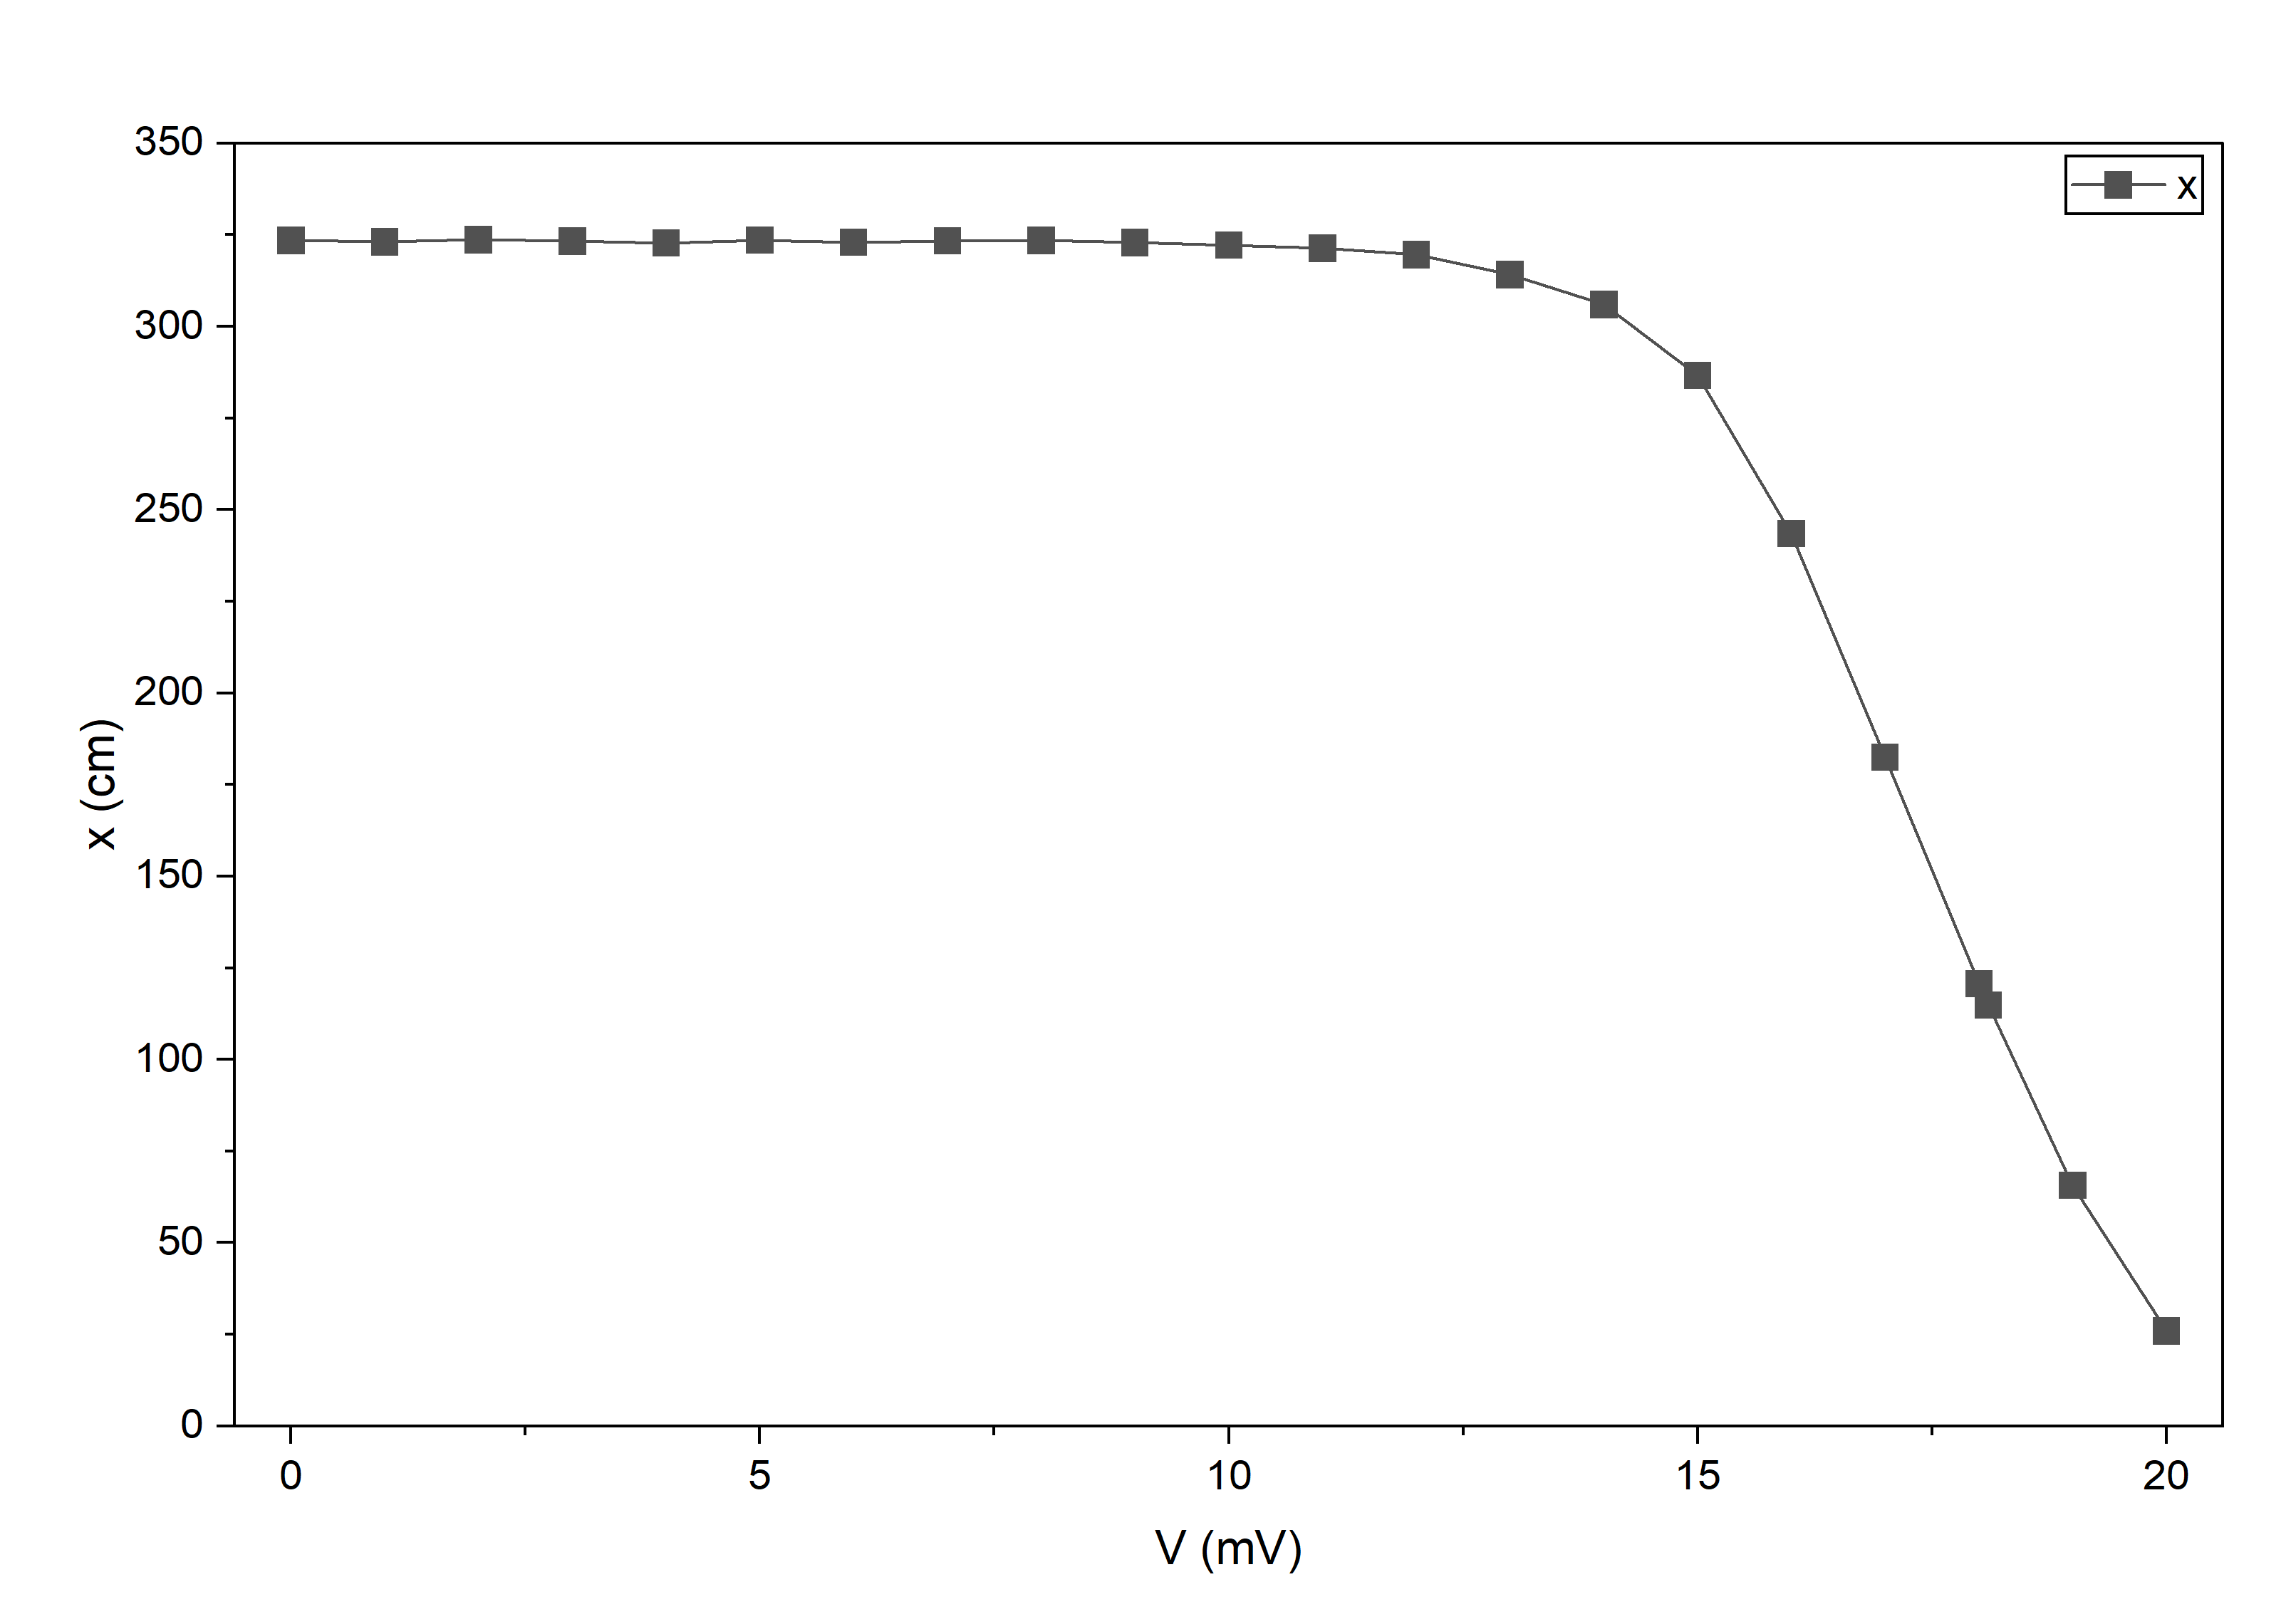
\includegraphics[width=0.8\textwidth]{4.png}
		\caption{$V-x$ 曲线}
		\label{fig:chart3}
	\end{figure}

	对比图1左的 $B-x$ 曲线可见，两条曲线形状相似，均在螺线管中心处达到最大值，在螺线管中保持几乎不变的稳定数值，并在边缘快速减小，符合磁场变化规律。因此可以认为 $V-x$ 曲线反映 $B-x$ 曲线的特征。由原理可知，二者仅相差倍数。

	计算得 $V_{x=l}/V_{x=0} = 114.82/323.5 = 0.355$，与理论值 $0.5$ 存在一定差异，可能原因包括探测线圈位置误差、环境干扰等。

	\end{enumerate}
	
	
	\section*{\textbf{八. 误差分析}}

	\begin{itemize}
    \item 螺线管的非理想性： 实际使用的螺线管并非无限长、单层且紧密绕制，其几何尺寸和绕制工艺会影响磁场的均匀性和分布，导致与理论公式的偏差。

    \item 几何参数测量误差： 螺线管的总匝数$N$、半径$R$、长度$2l$，以及探测线圈的匝数$N_1$、半径$r_1$等的测量可能存在误差，这些参数直接影响理论和实验B值的计算。
    
    \item 位置测量误差： 确定探测线圈中心沿轴线的位置$x$，特别是精确确定螺线管中心($x=0$)和管口位置($x=l$)存在一定难度，读数直尺的精度也有限。轴线对准误差也会影响测量结果。
    
    \item 电测量仪器误差： 电流表和电压表的读数误差、精度以及交流信号的有效值测量误差会影响$I$和$V$的准确性。

    \item 环境磁场干扰： 实验环境中的地磁场或其他电磁设备产生的杂散磁场可能对测量结果造成干扰，尽管交流磁场测量对外来的恒定磁场不敏感，但其他交流磁场源可能产生影响。


\end{itemize}

	\section*{\textbf{九. 思考题}}

	本实验可进行哪些方面的改进,以减小测量误差?
	\begin{itemize}
		\item 使用更高精度的测量仪器，如更精确的电压表和电流表。
		\item 精确测量螺线管和探测线圈的几何参数（匝数、半径、长度）。
		\item 对于$x$坐标的测量，可以使用更精确的定位装置。
		\item 多次测量取平均值，减小随机误差。

	\end{itemize}
	
	\section*{\textbf{{十. 实验结论}}}

	本实验通过测量螺线管轴线上的感生电动势，研究了螺线管磁场的性质：
	\begin{itemize}
		\item 在螺线管中心处($x=0$)，感生电动势$V$与通过螺线管的交流电流$I$近似呈线性关系，并且与交流电的频率$f$近似呈正比，这与电磁感应定律的理论预期相符。
		\item 沿螺线管轴线测量感生电动势$V$的分布，发现$V$（代表磁感应强度$B$）在螺线管中心区域近似均匀，并在靠近螺线管两端时显著下降。这一分布趋势与理论上有限长螺线管轴线磁场的分布规律定性一致。
		\item 实验测得的管口位置($x=l$)感生电动势与中心位置($x=0$)感生电动势的比值$\frac{V(l)}{V(0)} \approx 0.355$，与理论存在一定差异。可能由于实验误差和螺线管的非理想性所致。
	\end{itemize}

\end{document}